\section{VaRTOS}
In this section we present VaRTOS---a variability-aware architecture and corresponding extensions to the FreeRTOS \r{cite here} kernel for optimizing application-wide utility.  In doing so, we will introduce models for heterogenous tasks that comprise an application as well as corresponding utility functions. 

\subsection{Task Modeling}
We start first by introducing an \emph{application} $A$ as a set of \emph{tasks} $\{T_1, T_2, \ldots, T_n \}$, where each task represents a periodic subprocess of $A$.  It is assumed that a task $T_i$ will add an increase in utility $\delta u_i$ when given additional active compute time, $\delta T_{a,i}$. Here, $u_i$ is a utility function specific to task $T_i$ and analogous to quality of service (QoS).  Whereas some efforts take the stance that the $u_i$ should be provided by the developer (\cite{green2010} for example), we advocate offloading the burden to the OS itself.  In doing so, we will assume that $u_i$ is a monotonically non-decreasing function of active computation time $T_a,i$ or, equivalently, the duty cycle ratio specific to $T_i$ denoted $d_i$.  Tasks will offer varying degrees of utility for different $d_i$, and so some degree of user input is required to guide the optimization routine in distributing active time in an efficient manner.  To incorporate this user input, we introduce the concept of a task \emph{knob}.

\noindent\textbf{Task Knobs}: 
In order to tune the active time used per task and thus the task-specific duty cycle ratio $d_i$, we introduce the notion of task knobs denoted $k_i$, with the intuition that increasing $k_i$ will increase $T_{i,a}$, $d_i$, and $u_i$.  In practical terms, a task knob is a variable that will govern either (1) the period of a task or (2) the frequency with which a task is activated. We argue that the vast majority of tasks found in embedded applications will fall in one of these two classes, and those that require both frequency and period modulation can often be divided into two legal subtasks glued together with inter-process communications. For example, those that fall in class 1 include variable length sensing tasks, listening for inbound communication, and variable length processing chains.  Those that fall in class 2 include variable frequency transmission, variable frequency sensor sampling, time synchronization handshaking, control and actuation events, and more.  

Task knobs are created by passing a variable pointer to the OS, allowing direct manipulation of knobs by the optimization routine.  In addition, the developer specifies a minimum and maximum knob value, $k_{i,min}$ and $k_{i,max}$. The value $k_{i,min}$ specifies the minimum amount of work $T_i$ must do in order for it to be useful. Below this value, a task offers no utility.  The value $k_{i,max}$ specifies a value at which increasing $k_i$ further will yield only marginal or no added utility.  As an example, a radio transmission task may be useless if it does not meet a certain latency requirement, but usefulness may plateau at some frequency governed perhaps by the physics and time response of the event being sensed. 

\noindent\textbf{Interpolating Utility}: given $k_{i,min}$ and $k_{i,max}$ we construct a utility function $u_i = f(d_i)$ as a logistic (Sigmoid) function of the form 

$$
u_i(d_i) = {1\over{1 + e^{-c_id_i}}}, ~~c_i \ge 0
$$

We require only the convex portion of the Sigmoid function, choosing $u_i(d_i)$ to be of the particular form

\begin{equation}
u_i(d_i) = { 2\over { 1 + e^{-c_id_i }} }- 1, ~~c_i \ge 0
\label{eq:util}
\end{equation}

Here, $c_i$ governs the convergence rate of $u_i$ from the minimum utility to the maximum utility and is calculated as a function of $k_{i,min}$ and $k_{i,max}$ such that 99\% of the utility has been reached by $k_{max}$.  Increasing the percentage of $u_{i,max}$ realized by $k_{i,max}$ has the effect of arbitrarily steepening the utility curve. The constant $c_i$ can then be calculated from Equation \ref{eq:util} as

\begin{equation}
c_i = { -log\left( {2\over \epsilon + 1} - 1 \right) \over d_{i,max} - d_{i,min} }, ~~\epsilon = 0.99
\label{eq:c}
\end{equation}

Finally, each utility curve can be arbitrarily scaled by a priority scalar $p_i$ for tasks with intrinsically higher utility than others. Figure \ref{fig:util} shows three example utility curves corresponding to three tasks with various priorities and duty cycle ranges (resulting from various $k_{i,min}$ and $k_{i,max}$). 

\begin{figure}
\centering
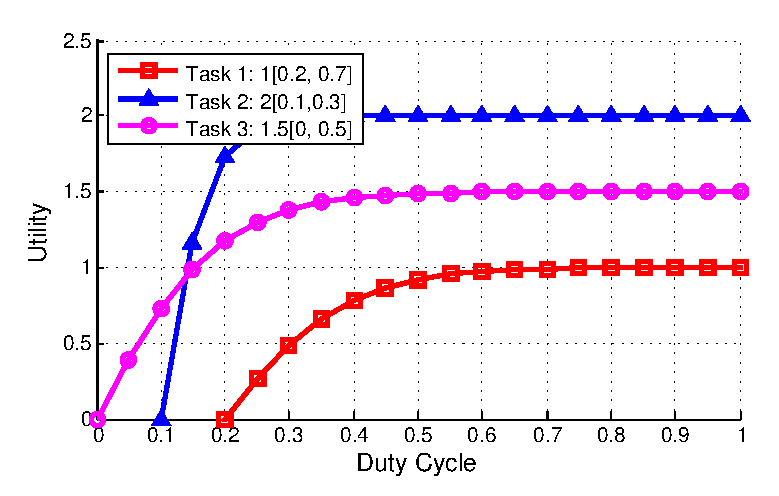
\includegraphics[width=1\columnwidth]{figures/utilityfunctions.eps}
\caption{\label{fig:util}Example utility curves. Task 1 has priority scalar 1 with useful range $d_i = [0.2, 0.7]$, task 2 with priority scalar 2 and so forth. }
\end{figure}

\noindent\textbf{Learning the $k_i \rightarrow T_{i,a}$ Relation}: Because the developer has free reign to use the knob $k_i$ for each task as desired, the function mapping $k_i$ to active time $T_{i,a}$ and thus $d_i$ is not known \emph{a priori}. Instead, the transformation $\mathcal{K}_i$ that maps $k_i$ to $T_{i,a}$  is assumed linear and is learned through regression at runtime. Should the developer misuse $k_i$ in a way that is nonlinear or results in non-increasing values of $T_{i,a}$, the optimization routine will suffer. Active time per task can be measured using hardware timer snapshots at the context swap level or other mechanisms described later in the text.  Given a method for measuring $T_{a,i}$, $\mathcal{K}_i$ is arrived at by systematic perturbation of $k_i$ within the range $[k_{i,min}, k_{i,max}]$. Specifically, $k_i$ is repeatedly increased by $\Delta = {k_{i,max} - k_{i,min} \over N}$ where $N$ is the number of points in the regression, kept sufficiently low ($N = 3$ in our case) to minimize memory footprint.  Between each perturbation in $k_i$, the task is allowed to run for a time period sufficiently long enough to capture active time measurements even for tasks with very infrequent activity.  In the applications presented here, this supervisory period is set at 1 hour. Dividing active time accumulated per task by the supervisory interval yields task-specific duty cycle ratios, $d_i$. 

\subsection{System-wide Duty Cycle}
Distributing active time per task assumes that we can afford a certain system-wide active time per supervisory interval, or equivalently that the system is governed by an optimal duty cycle $d^*$.  Arriving at $d^*$ is done in the same way as set forth in \cite{wanner2011} with the exception that the active and idle/sleep powers ($P_a$ and $P_s$) are learned at runtime.  The optimal duty cycle $d^*$ is calculated as a function of $P_a, P_s$, and $\pmb{f}_T$, where $\pmb{f}_T$ is the probability density function of the temperature for the location where the system is to be deployed. Given these quantities, $d^*$ can be found as a solution to the optimization problem

$$
d^* = \max ~~{d}~~\text{subject to:}
$$
\begin{equation}
\sum_Tf_T\left[dP_a(T) + (1-d)P_s(T)\right] \le {E\over L} = \bar{P}
\label{eq:opt}
\end{equation}

That is, maximize $d$ such that the lifetime and energy constraints are met.  Here, $E$ and $L$ are the energy and lifetime specifications and $\bar{P}$ is the average power needed to obtain lifetime $L$. The optimal solution to Equation \ref{eq:opt} can be obtained algebraically as shown in \cite{wanner2011}:

\begin{equation}
d^* =  { E - L\bar{P_s} \over L(\bar{P_a} -\bar{P_s}) } 
\end{equation}

Where $\bar{P_a}$ and $\bar{P_s}$ are temperature-averaged power quantities. 

\subsection{Optimizing Utility}
Because we have chosen $u_i$ to be a logistic function, we can use a greedy approach when optimizing utility.  The optimization routine will be a two step process: (1) attempt to assign the minimum duty cycle $d_{i,min} = \mathcal{K}_i(k_{i,min})$ needed for each task to yield utility in order of decreasing priority, and (2) continue distributing utility to the task 


\begin{figure}
\centering
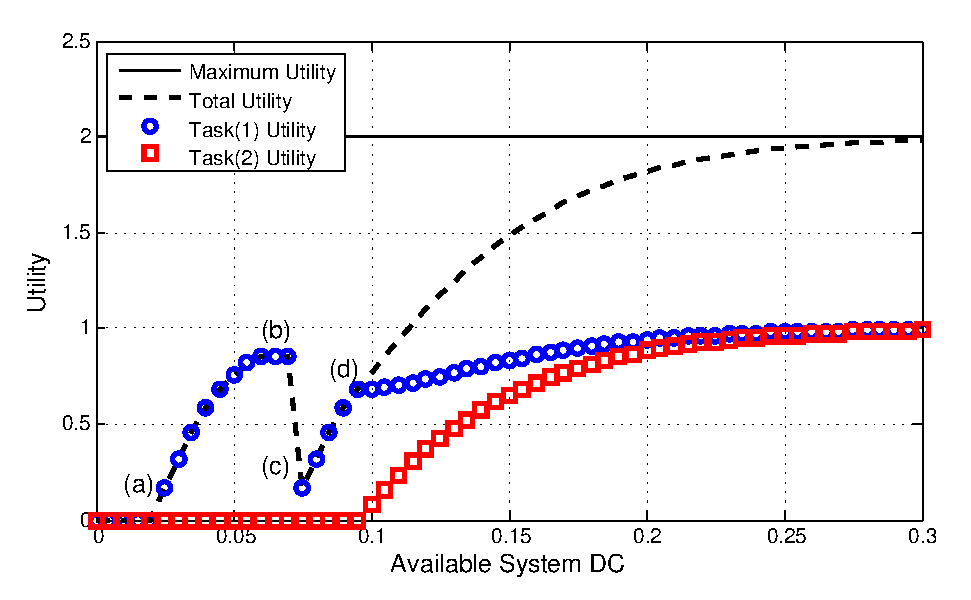
\includegraphics[width=1\columnwidth]{figures/optimalDCexample.eps}
\caption{\label{fig:optimaldc_mult}optimizing shit}
\end{figure}

\begin{figure}
\centering
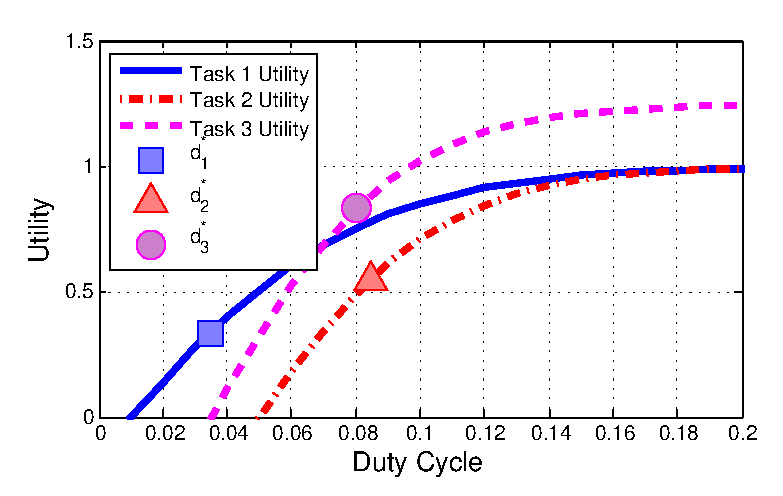
\includegraphics[width=1\columnwidth]{figures/utilanddc.eps}
\caption{\label{fig:utilanddc}optimizing shit}
\end{figure}

\begin{figure*}
\centering
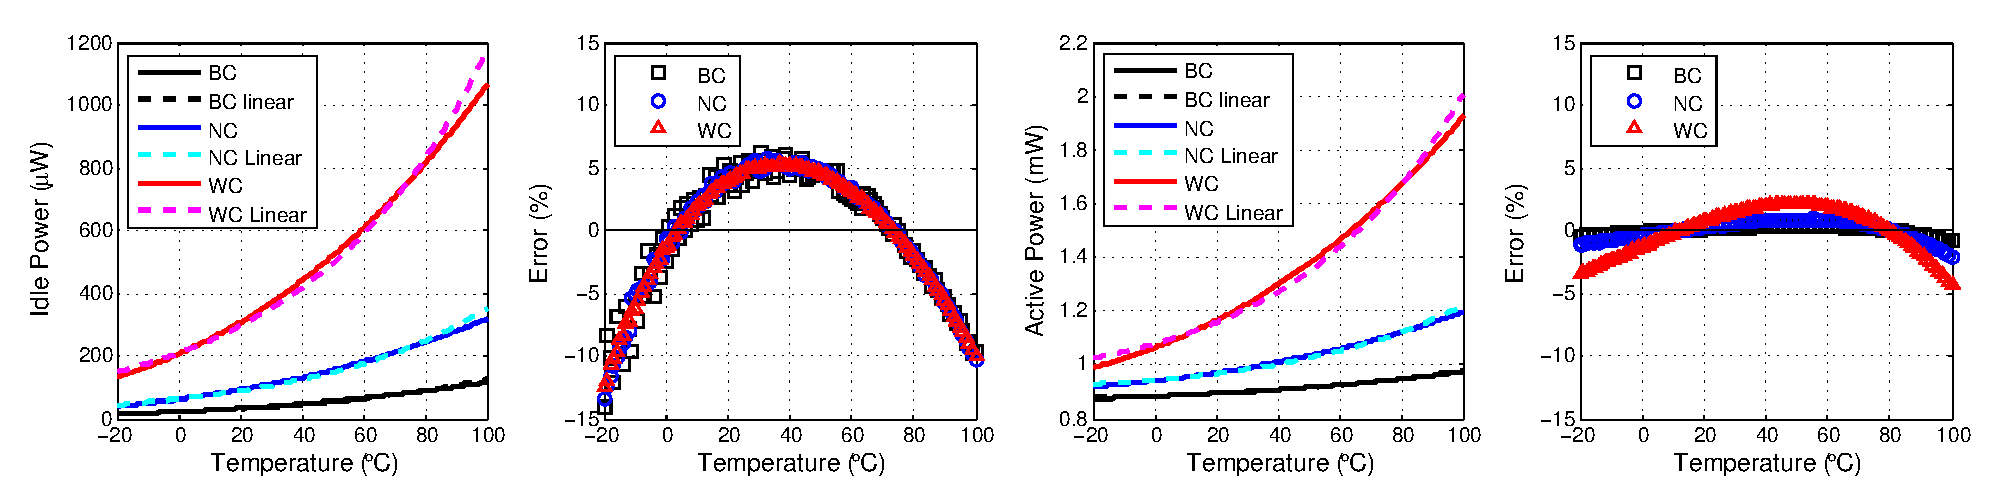
\includegraphics[width=1\textwidth]{figures/powerlearning.eps}
\caption{\label{fig:powerlearning}Learning power....}
\end{figure*}


%% Algorithm
\begin{algorithm}
 \SetAlgoLined
 \KwData{$u_a(d) \forall a \in A, ~d^*_T$}
 \KwResult{$d^*_a$ }
 $d_{remaining} \leftarrow d^*_T$.  \\
 Assign min knob values:\\
 \For{$a \in A$}{
 	\eIf{$d_a(k_{min}) < d_{remaining}$}{
 	$d_a = d_a(k_{min})$\\
	$d_{remaining} \leftarrow d_{remaining} - d_a$
 	}{
 	stop
 	}
 }
 Divvy up remaining duty cycle fairly:\\
 \While{$d_{remaining} > 0$}{
 	Find highest marginal utility:\\
	$maxM.U. \leftarrow 0$\\
	$numMax \leftarrow 1$\\
	 \For{$a \in A$}{
	 	\eIf{$m(a) > maxM.U.$}{
			$maxM.U. \leftarrow m(a)$
			$numMax \leftarrow 1$
		}{\If{$m(a) == maxM.U.$}{
			$numMax \leftarrow numMax + 1$
		}
		}
	 }
	 
	 Increment task duty cycles:\\
	 $d_{requested} \leftarrow \delta \cdot numMax$\\
	 \If{$d_{requested} > d_{remaining}$}{
	 	$d_{requested} \leftarrow d_{remaining}$
	 }
	 \For{$a \in A$}{
	 	\If{$m(a) == maxM.U.$}{
			$d_a \leftarrow d_a + d_{requested}/numMax$
		}
	 }
 }
 \caption{Greedy duty cycle optimization}
\end{algorithm}

\subsection{Instance Modeling}
including sleep and active power, and musings on learning the temperature profile etc.



\subsection{Operation}
Talk about what happens in steady state, how we check for errors, what happens when errors become large, etc. 

\begin{figure}
\centering
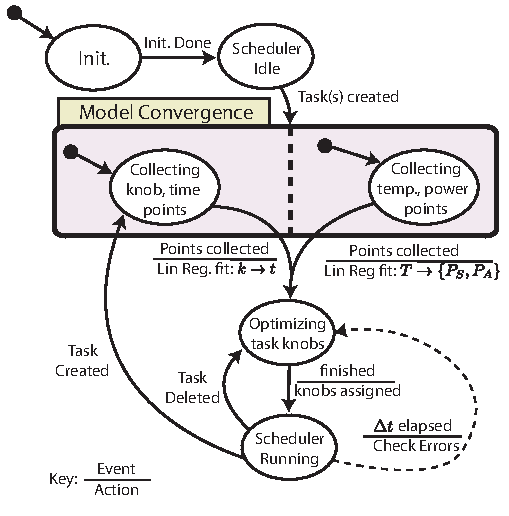
\includegraphics[width=1\columnwidth]{figures/statechart.pdf}
\caption{\label{fig:state chart}state chart}
\end{figure}

\begin{figure}
\centering
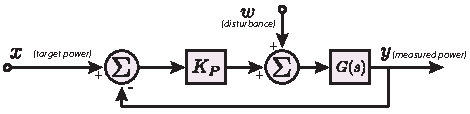
\includegraphics[width=1\columnwidth]{figures/controlloop.pdf}
\caption{\label{fig:state chart}state chart}
\end{figure}




